\documentclass[final,a4paper,twoside,11pt,onecolumn]{report}
% if you use "report", you get a seperate title page
%\documentclass[final,letterpaper,twoside,12pt]{article}
%
% Längd-infor: N Tsiftes rapport är 35 sidor lång (exkl. bibliografi och appendix) och är typsatt i 11 punkter

\usepackage[utf8]{inputenc} 
%\usepackage[swedish]{babel}prettyref
\usepackage{fancyhdr}
\usepackage{graphicx}
\usepackage{empheq}
\usepackage{natbib}
\usepackage{url}
\usepackage{nameref}
%\usepackage{showkeys}
\usepackage{prettyref}
\usepackage{varioref}
%\usepackage{cleveref}
\usepackage{hyperref} % To be loaded AFTER cleveref
%\usepackage[margin]{fancyref}

\DeclareGraphicsExtensions{.pdf,.png,.jpg,.jpeg}
\graphicspath{ {bilder/} }

% For prettyref
\newrefformat{eq}{\textup{(\nameref{#1})}}
\newrefformat{lem}{lemma \nameref{#1}}
\newrefformat{thm}{theorem \nameref{#1}}
\newrefformat{cha}{chapter \nameref{#1}}
\newrefformat{sec}{section \nameref{#1}}
\newrefformat{tab}{table \nameref{#1} on page \pageref{#1}}
\newrefformat{fig}{figure \nameref{#1} on page \pageref{#1}}

\def\Figref Figure:#1:{\figref{fig:#1}}
\newrefformat{Fig}{Figure~\Figref#1:}

% For suppressing the chapter label. Not working atm.
%\renewcommand{\chaptername}{}
%\renewcommand{\thechapter}{}

\begin{document}
\author{Vilhelm~Jutvik \thanks{To everyone at SICS and the NES group}}
\date{\today}
%\title{The adaption of the IKEv2 protocol for The Internet of Things MS Thesis project plan}
\title{IPsec for the Contiki OS}

\maketitle

% 
% en beskrivning av det problem som angripits: problemformulering och problemstrukturering;
% en beskrivning av de metoder som använts för att lösa problemet;
% tolkning och diskussion av resultat - en analys av hur väl problemet lösts;
% om problemet ej lösts fullständigt, en beskrivning av de troliga orsakerna till detta - även negativa resultat och erfarenheter kan ofta vara värda att rapportera (så slipper andra göra om det);
% innehållsförteckning;
% litteraturförteckning.
% Vidare skall
% 
% de egna metoderna granskas kritiskt;
% en jämförelse med andras arbeten rörande liknande problem ingå.

\begin{abstract}
In this the work the author explores...
\end{abstract}

\setcounter{tocdepth}{4}
\tableofcontents

\chapter{Populärvetenskaplig sammanfattning}
nödvändig bakgrundsinformation för en allmänbildad läsare som inte nödvändigtvis är specialist inom området;

hot and cold mediums

\chapter{Introduction}
\label{cha:intro}
The Internet has revolutionized communication. The author would like to argue that this happened because it drastically lowered the cost of communication by removing interface barriers, unifying standards and organizations. Internet is cheap while legacy, purpose-made, communication networks are expensive (e.g. consider the PSTN\footnote{Public Switched Telephone Network, your ordinary phone}). These lowered costs allowed people to send and receive information at an enormous rate, creating new types of medias and services such as the blog, the social network, the search engine etc. Because of these benefits, we try to expand the Internet, and now strides are being made to connect the objects that we surround ourselves with, creating what's commonly called he `Internet of Things' (abbreviated as IoT). It's a vision of an extended Internet where household objects (radiators, lighting etc), sensors and actuators in industrial machinery, cars etc are put `online'. Data is primarily sent and received by radio as cables are expensive to install and maintain.

The underlying motivation as to why we want to communicate with things are that they and their surroundings matters to humans. A thing such as freezer can notify building management when its about to break down and notify building management before the food is spoiled. Data from the vibration sensor in the bridge helps the engineer to model its health and plan maintenance. A thing can also help another thing, e.g. the temperature sensor telling the radiator to turn as the temperature is falling.

% This is of importance to humans as its believed that the IoT will greatly reduce the cost for communication thing to thing and man to thing. This enables more information to be shared, and more information usually translates into a better understanding of the environment, which translates into a more efficient world. An example of this would be an Internet-connected temperature sensor in a room which gives the IoT-enabled radiators a better idea about when and how much heat to apply.

Unlike a regular host on the Internet (e.g. a PC) an IoT device is often purpose-made for a few single tasks (e.g. measuring the temperature in the example above). Data is usually sent and received over radio. This allows the computer's electronics to be small, cheap and consume little power, so little that it can be run of a non-rechargeable battery for the system's entire lifetime. This set of technological characteristics are what commonly characterize the IoT.

%The promise of cheap, ubiquitous and easily installable computers bundled with the Internet's ease of communication is what fuels the vision of an Internet of Things.

Contiki is small and resource efficient operating system that tries to address the above requirements. With only 35 kB of ROM and 8 kB RAM it provides an IP stack as well as multitasking. On the multitude of platforms officially supported, the hardware is often composed of a small 16-bit CPU, a small non-rechargeable battery and a radio operating in the 2.4 GHz ISM band FIXCORRECT. Developed mainly at SICS, the OS have gathered a large following around the world, only surpassed by its relative TinyOS. Naturally, Contiki is the primary research platform for IoT at SICS, and is why the work of this thesis is based upon it.

As the IoT will control and monitor sensors as well as machines in our surroundings, security is a natural concern. Internet (more specifically, the IP protocol) by itself does not offer any security guarantees by default. This is especially true in the IoT world where the physical layer often is provided by radio. Therefore, this thesis will explore the possibilities of implementing the IPsec security extension of the IP-protocol in the Contiki OS. This will bring methods to secure communications to the IoT, that are also compatible with vast parts of the Internet.


%Although this allows communication with the rest of the Internet, it cannot be done in privacy. Any host in the path of a message between it and any other host can read, stop or manipulate the data. This is problematic if the IoT device measures or controls something deemed important to humans, such as a door lock or a motion sensor in a burglar alarm. Therefore the author have investigated whether or no it's feasible to implement support for an Internet standard that enables hosts to communicate securely over the Internet; IPsec. IPsec is an IETF\footnote{Internet Engineering Task Force} standard that is a part of IPv6, the coming replacement to the current IP protocol. This thesis outlines its design, implementation and evaluation of this standard and its utility in the Contiki OS.



%  For example;  As the hosts (computers) usually are located inside, or in the direct vicinity of the object of interest,    power is usually supplied by a small non-rechargeable battery and communicates by radio.\\
% \\
%  This implies that said devices must be able to use the same protocols and standards as the rest of the Internet. One such piece is the suite of security features offered by the IP protocol, called IPsec.\\
% \\
% Contiki is an OS for devices running on the Internet of Things. It features an implementation of the IP protocol and several other Internet standards. The purpose of this work is to add yet another standard to it; IPsec. IPsec is an extension to the IP protocol that enables hosts to communicate securely over the Internet. Naturally, there are several implementations of IPsec readily avaible, but we can't use them since they don't fit. IoT devices that runs Contiki are usually very constrained in memory as well as CPU, but above all, energy is most important. The typical IoT -device is battery powered. Because of this, the result of the work must be able to save resources whereever possible, 

\section{Problem statement}
As the IoT will control and monitor sensors as well as machines in our surroundings, security is a natural concern. Internet (more specifically, the IP protocol) by itself does not offer any security guarantees by default. This is especially true in the IoT world where the physical layer often is provided by radio. Any device with suitable radio equipment can read IP-packets destined for others, create and send packets while imposing as another host and manipulate data in transmissions destined for somebody else. This is problematic if the IoT device measures or controls something deemed important to humans, such as a door lock or a motion sensor in a burglar alarm. When receiving a message in the case of the former, the host controlling the door lock wants to assert that: the identity of sender is correct; that the message have not been tampered with; and preferably, it should be encrypted so that no other host except the addressee can read it. At the same time, the technology enabling this must be supported by the lock (the IoT device) and the other host, which might be any type of machine anywhere on the Internet. IPsec is one of many similar standards designed to solve these problems.

The difficulty of the work lies in making an implementation that is compatible with other hosts on the Internet (enabling communication), fulfilling the security requirements (correctness) while simultaneous assuring that the code is small enough to fit in the limited memory. This also relates to energy requirements, especially in the context of cryptography which is heavily used by IPsec, as computations consumes a sizable part of an IoT host's energy budget.

\section{Research question}
Can IPsec and IKEv2 be implemented within the current hardware boundaries while still being interoperable with other Internet hosts?
 
%There are several different solutions to these problems. One of them is IPsec, which is the standard that the author has chosen to implement for the Contiki OS. The main hurdle 
%Solutions to these problems are provided by several different stan
%These problems are solved by several different standards
%The author's hypothesis is that the IPsec extension of the IP protocol can fulfill these criteria. 

%\section{Hypothesis / Proposed solution}
%The author has worked with the hypothesis that the aforementioned requirements can be fulfilled by the IPsec standard. It's a well estbalished protocol and most of the hosts connected to the Internet already has supported it for a number of years. The purpose of investigating whether or not it's feasible to solve this problem by implementing an existing Internet standard in the Contiki OS.


%implement support for an Internet standard that enables hosts to communicate securely over the Internet; IPsec. It's an extension of the replacement for the current IPv4 Internet Protocol, IPv6. The 

%listen in the network can send For example, consider the case of the door lock that is connected to the Internet via IoT. Anyone device which  When it receives a message telling it to unlock it wants to assert the identity of the sender, know 

% The goal of this thesis is the investigate the feasibility of using IPsec in the Contiki operating system. This implies that the software implementing the standard should not only fit on the device's limited ROM memory, but be demonstrated to actually do something useful.

% IPsec is an Internet standard for secure host-to-host communication. Some of its benefits have been mentioned above, but can it be implemented in Contiki?
%will endow Contiki with secure communication facilities, but at what cost, if it's possible at all? 

    %    Kan IPsec / IKE implementeras i Contiki på den här begränsade hårdvaran?
    % -> Vad krävs för att contiki-implementation / min implmenettation ska anses vara användbar?
    %          * Bevisa att den kan upprätta och hantera IKE -anslutningar
    %          * Minnes och beräkningskraft
					
\section{Method}
Much of the research in IoT is carried out by experiments because of the highly applied nature of the field. Indeed, most of the Internet as-of-today, was constructed on the basis of principles surmised from experiments. Therefore, the author decided to  implement the various components that makes up a functional IPsec system and then test them. The tests were carried out by subjecting the system to common communication scenarios with other IPsec-enabled Internet hosts: handshaking a new secure connection; receiving and transmitting packets with various security policies applied; housekeeping of connections. The success or failure of the test is determined if it worked, or if it succeeded, how well it did so. Finally, memory consumption and cpu time is measured for the different tasks. It's the results of these tests that will form the basis of the evaluation of the 1) quality and workmanship of the implementation 2) suitability of IPsec for IoT in general.

\subsection{Development process}
The source code was managed using the Git source code revision system. Development was organized in such a way that the project was run in one branch\footnote{Git branches are similar in concept to those in other SCMS. ...} (hereafter called \emph{develop}) parallel to Contiki's master branch. Important patches / changes that occurred in Contiki while the development was underway could thus simply be fetched / merged into \emph{develop}. Patches in develop that proved  was then merged in from the 

\section{Limitations}
Firstly, the purpose of this work is to answer the questions raised in the problem statement, not to create an implementation that's ready for production use. Thus, parts of the standard that are not necessary to meet this end can be omitted. This also includes parts that are labeled as REQUIRED in the standard documents, as they're only necessary if you strive towards full compliance, which in terms of features arguably is superset of that of interoperability.

\section{Alternative Approaches}
There are many ways of securing communication in a computer network, far too many to review in this section. What follows is a swift review of the closest alternatives for security in IoT networks. A thorough review and comparison will be made of these in the discussion towards the end of this thesis.

The traditional approach in the IoT world has been to secure communication by using the IEEE's 802.11.4 link layer and its security features. There are also plenty of research articles outlining completely new security schemes, but none of these have made it into and IETF standard as far as the author is aware. Another alternative is the IETF's TLS protocol\footnote{The TLS protocol is a successor to SSL} that operates next to the application layer, but no implementation of that has been completed as of today to the best of the author's knowledge.

A final possibility would be to come to a conclusion by using analysis. Supposing that the main obstacle to a functional solution is that of ROM, RAM, CPU speed and energy requirements. As one can assume the cryptographic libraries to consume the majority of the resources, one can arrive at an approximation for the hardware requirements by benchmarking them stand-alone. This would certainly help in arriving at an upper bound for the hardware requirements, but the analysis would not tell us anything about the operational problems and benefits that a complete implementation would.

%These can be ordered by the network layer\footnote{The notion of network layers is derived from the idealized OSI-model in which network protocols are ordered in a stack of seven layers.} at which they operate.

%\paragraph{The link layer} can provide authentication, confidentiality and integrity if using the IEEE 802.15.4 radio link layer, commonly employed in IoT systems. The benefits are that it's transparent to 
	
%	Alternative approaches: Beräkna storleken på kryptobibliotek mm + skatta kodkraven på andra delar, summera sedan
%	Scientific contributions: Evaluerin
%	Report structure

\section{Scientific Contributions}
This report makes three scientific contributions. The first is the demonstration of that it's feasible to implement IPsec with dynamic key management and IKEv2 in the Contiki OS. The second is that it's possible to simplify the IPsec protocol in IPv6-IoT environments without sacrificing much in interoperability. The final is that IPsec's network-centric policy language is ill suited for ad-hoc, self-organized network environments, such as that created by the RPL\footnote{The Routing Protocol for Low-Power and Lossy Networks (RPL) is an IETF standard (RFC 6553) that creates dynamic routing topologies} routing protocol commonly used in conjunction with IoT.

\section{Report Structure}
The purpose of the \prettyref{cha:intro} is to give the reader an overview of the report. The next chapter, \nameref{cha:bg}, will begin by a discussion of the problems that are particular to the field of IoT and how Contiki is constructed. This will be followed by a brief recount of the background and design of IPsec, followed by an introduction to automatic keying and the IKEv2 protocol. In \prettyref{cha:doi} the author outlines how the IPsec standard is adapted to IoT and Contiki. Simplifications and omissions of features are explained and argued for. The design is then evaluated in \nameref{cha:eval} by measuring parameters such as time, energy and memory usage when sending and receiving data. Space will also be given to observations of a qualitative nature, such as how well the standard integrates with the Contiki OS. The author's opinions of the evaluation and suggestions for future work is given in \nameref{cha:fw}.


\chapter{Background}
\label{cha:bg}
The purpose of this chapter is to introduce the reader to the Contiki OS and the IPsec standard. A good understanding of these systems are necessary to understand the later \prettyref{cha:doi}.

\section{Contiki}
Contiki is an operating system designed for computers with severely constrained resources\cite{dunkels04contiki}. At the time of its original release in 2004 it was targeted at 8-bit micro controllers, ROM on the order of 100 kB and RAM less than 20 kB\citep[1]{dunkels04contiki}. Although the production costs of electronics certainly will continue to fall in future, this doesn't necessarily translate into a lesser interest in resource constrained operating systems such as Contiki - the lower prices can be used to produce more units instead of making existing devices more powerful. The choice of small devices such as the traditional 8- and 16-bit micro-controllers that has been the mainstay of Contiki since its inception\footnote{Examples of micro-controllers commonly used with Contiki are Texas Instrument's MSP430 architecture and Atmel's AVR 8-bit dito.}, is not just about cost, but also about power efficiency. Small chips have been, for various reasons, more energy efficient on a per cycle basis than heavier systems (e.g. the 32-bit  Cortex-M3 platform from the ARM Corporation). Having said that, this is set to change as the more powerful micro-controllers are becoming increasingly energy-efficient, a fact which we will address in the \prettyref{cha:fw}.

Having stated this, Contiki's greatest benefit is not that it's very compact, it's that it provides `a rich enough execution environment while staying within the limitations of the constrained devices'\citep[Introduction]{dunkels04contiki}. The `rich execution environment' is a reference to Contiki's capability to dynamically load and unload software, its multithreading, mesh networking\cite{tsiftes10rpl} and more, that are all designed to fit within the constraints, memory- as well as energy-wise (i.e. limit the number of execution cycles and keep peripherals such as the radio asleep). We will now review the most important of these features that makes Contiki a popular OS for IoT-devices.

\subsection{Multitasking}
Multitasking (concurrency) is provided in Contiki by the \emph{Protothreads} mechanism\cite{dunkels2005protothreads}. Before explaining its inner workings, the author will provide the reader with a short review of the problems associated with multitasking in resource constrained systems.

The motivation underlying protothreads is to provide the programmer with multitasking that is easy to use, easy to understand and low in resource consumption. Multitasking has traditionally been implemented in virtually all operating systems by the means of \emph{processes}. In such a model, each \emph{process} is associated with an executable, has its own private stack and memory, set of registers (etc) and can be interrupted (more specifically, \emph{preempted}), at any time by the operating system's \emph{scheduler} in order to run a kernel specific task or to \emph{schedule} another task. In all cases where a process is preempted, a \emph{context switch} has to take place where much of the CPU's registers are changed, caches flushed etc. This is unsuitable for constrained environments due to the massive memory overhead of a process structure, private stacks and the energy required for doing a context switch.

One approach to overcome these drawbacks while still allowing some form of multitasking was employed by another sensor network OS: TinyOS\cite{levis2005tinyos}. TinyOS allowed the programmer to achieve multitasking by implementing their programs as event driven state machines. The machines has no stack and can only keep state (i.e. data) that are implicitly declared as such. As the C programming language doesn't have any event primitives, an extension to C was developed and named \emph{nesC}\cite{gay2003nesc}.

Contiki took a different route and provided the programmer with a model that resembled the sequential programming style (which is believed to be more comfortable for the majority of developers)\footnote{The author found this reasoning to have merit after having participated in a course where application programming for TinyOS as well as Contiki was taught, having observed that the vast majority of his classmates preferred Contiki's Protothreads to TinyOS' nesC.}, but still benefitted from the efficiency of the event driven state machine.

\begin{figure}[h!]
   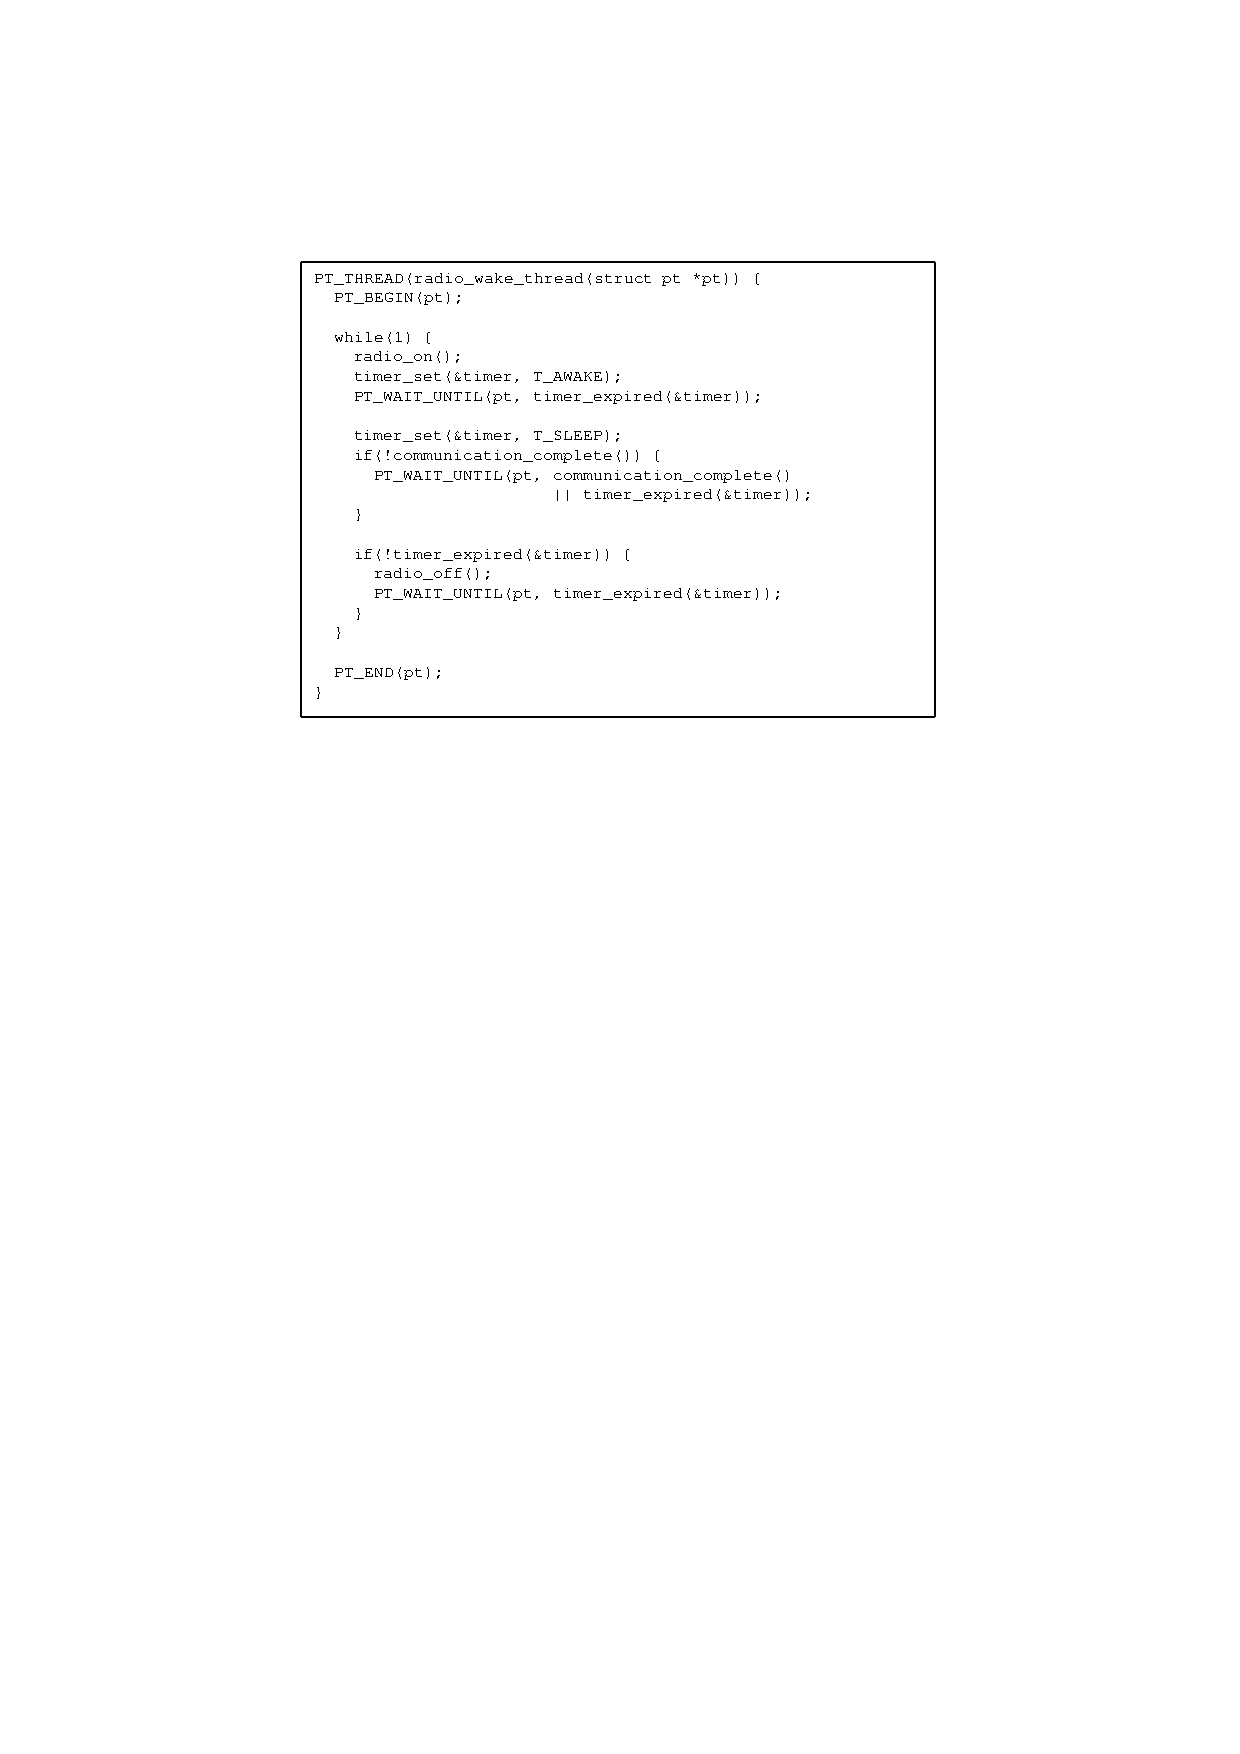
\includegraphics[width=0.9\textwidth]{dunkels-protothreads-example}
   \caption{Example code for a radio transmission program utilizing Protothreads. From \citep[p.7]{dunkels2005protothreads}. FIX: Check copyright!}
   \label{fig:ptexample}
\end{figure}

In figure \vref{fig:ptexample} a code example using Protothreads is shown, in which a radio is awaken at a set schedule to wait for check for transmissions. Protothreads uses a concept called \emph{conditional blocking} which can be explained in the following way: the execution can't leave the thread until a conditional blocking statement is reached (macros prefixed with `PT'). This can also be referred to as \emph{cooperative multitasking} as control can only leave a program when it voluntarily relinquish it.

As all Protothreads share the same stack and Contiki only needs to remember at which conditional to resume the thread, memory requirements can be as small as 2 bytes of RAM per thread. Furthermore, curiously enough, the `context-switching' mechanism can be wholly implemented using only the C switch control structure. This `quirk' of the C language was probably first discovered by Tom Duff\citep[p.10]{dunkels2005protothreads}\cite{wiki:duffs}.

%Programs written for an event-driven model typically have to be implemented as ex- plicit state machines. In contrast, with protothreads programs can be written in a se- quential fashion without having to design explicit state machines. To illustrate this, we return to the radio sleep cycle example from the previous section.

%\paragraph{Hardware support}
%From 8-bit to 32-bit Cortex M3. Requires bla bla ROM and RAM.

%Support for many 802.11.4 devices.


\subsection{IP networking}
UDP, TCP as well as ICMP over IPv4 and IPv6 are provided by the $\mu$IP stack, described in\cite{dunkels2003full}. The system is surprisingly robust given that its footprint amounts to only ~10 kB of ROM and a couple of hundred bytes of RAM: it fulfills all necessary host-to-host requirements stipulated in the relevant RFC documents\citep[p.4]{dunkels2003full} (e.g. flow and congestion control). The number of TCP connections and the size of the transmission / reception buffers are only limited by available RAM.

\begin{figure}
   \centering
   \begin{minipage}{.5\textwidth}
      \centering
      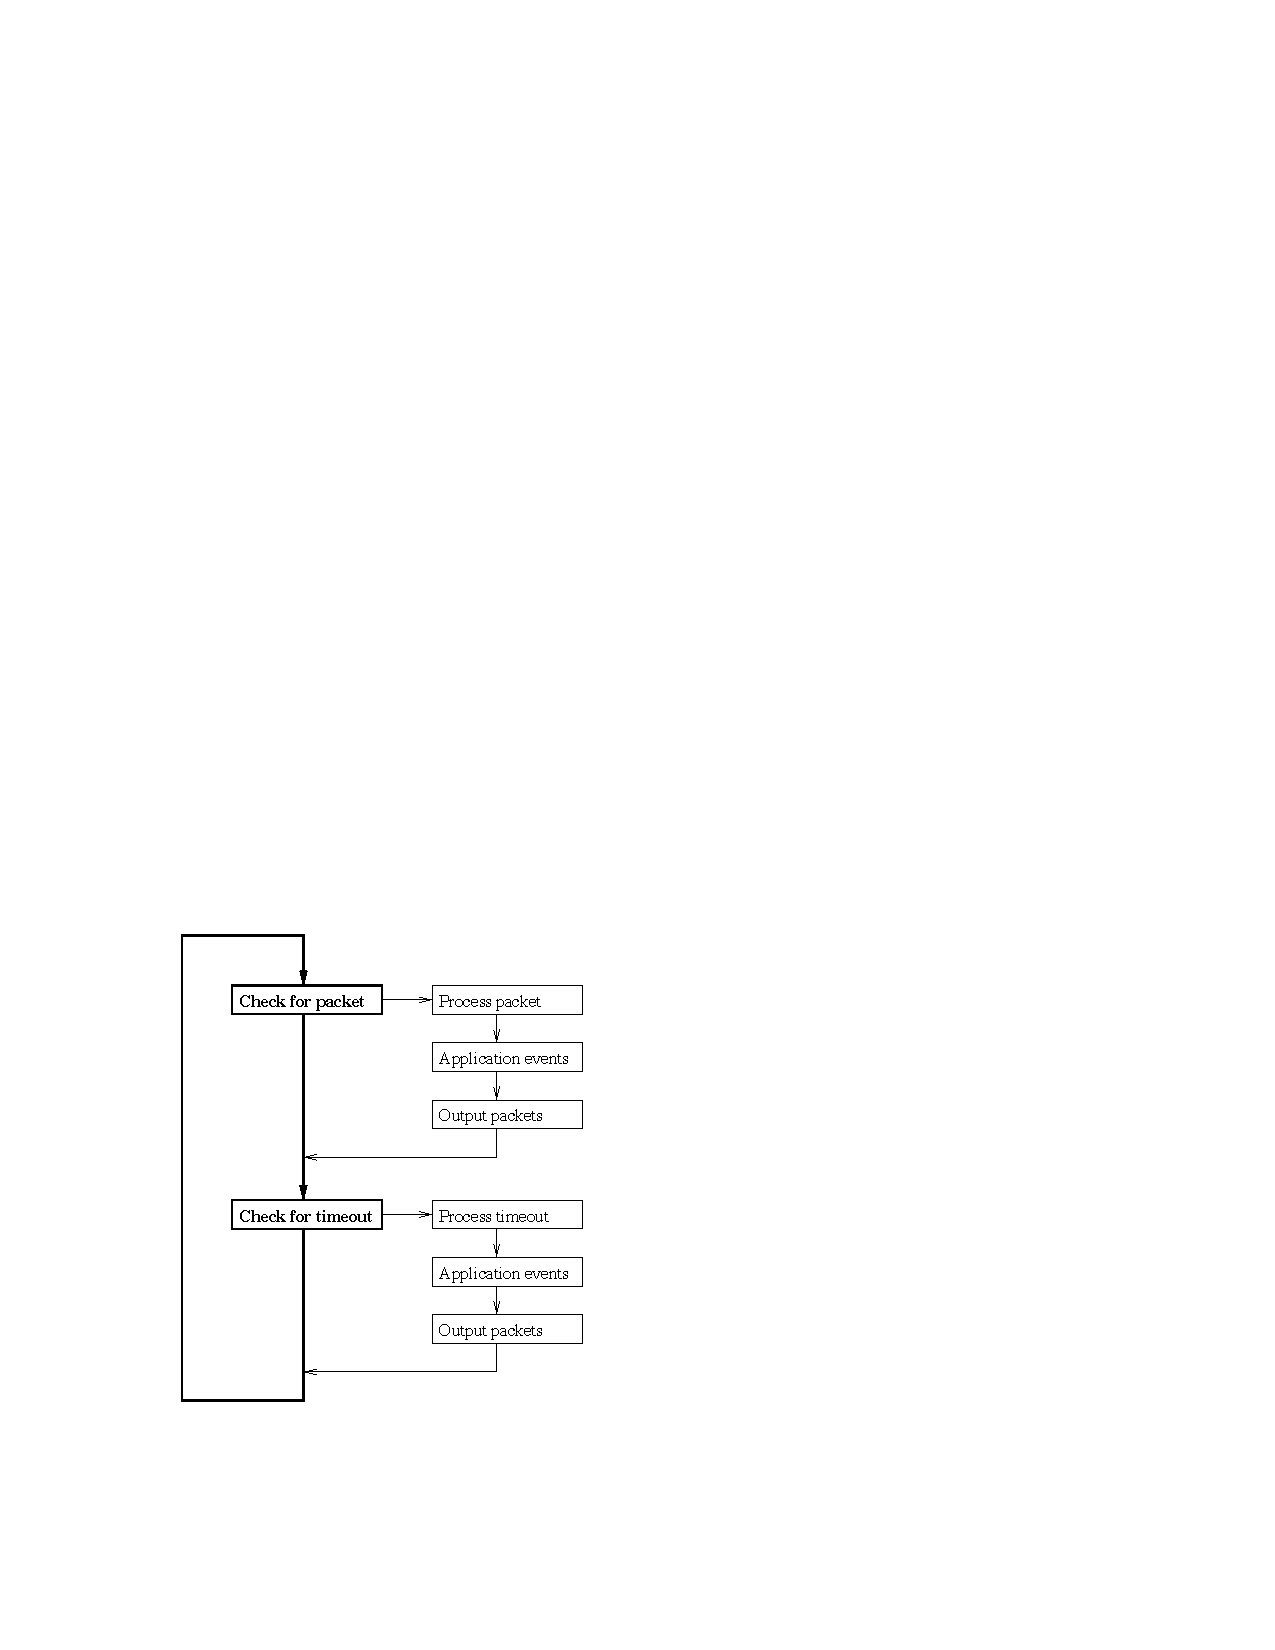
\includegraphics[width=.9\linewidth]{dunkels-uip-main_loop}
      \caption{$\mu$IP's main control loop. From \citep[p.6]{dunkels2003full}. FIX: Check copyright!}
      \label{fig:uip-ml}
   \end{minipage}%
   \begin{minipage}{.5\textwidth}
      \centering
      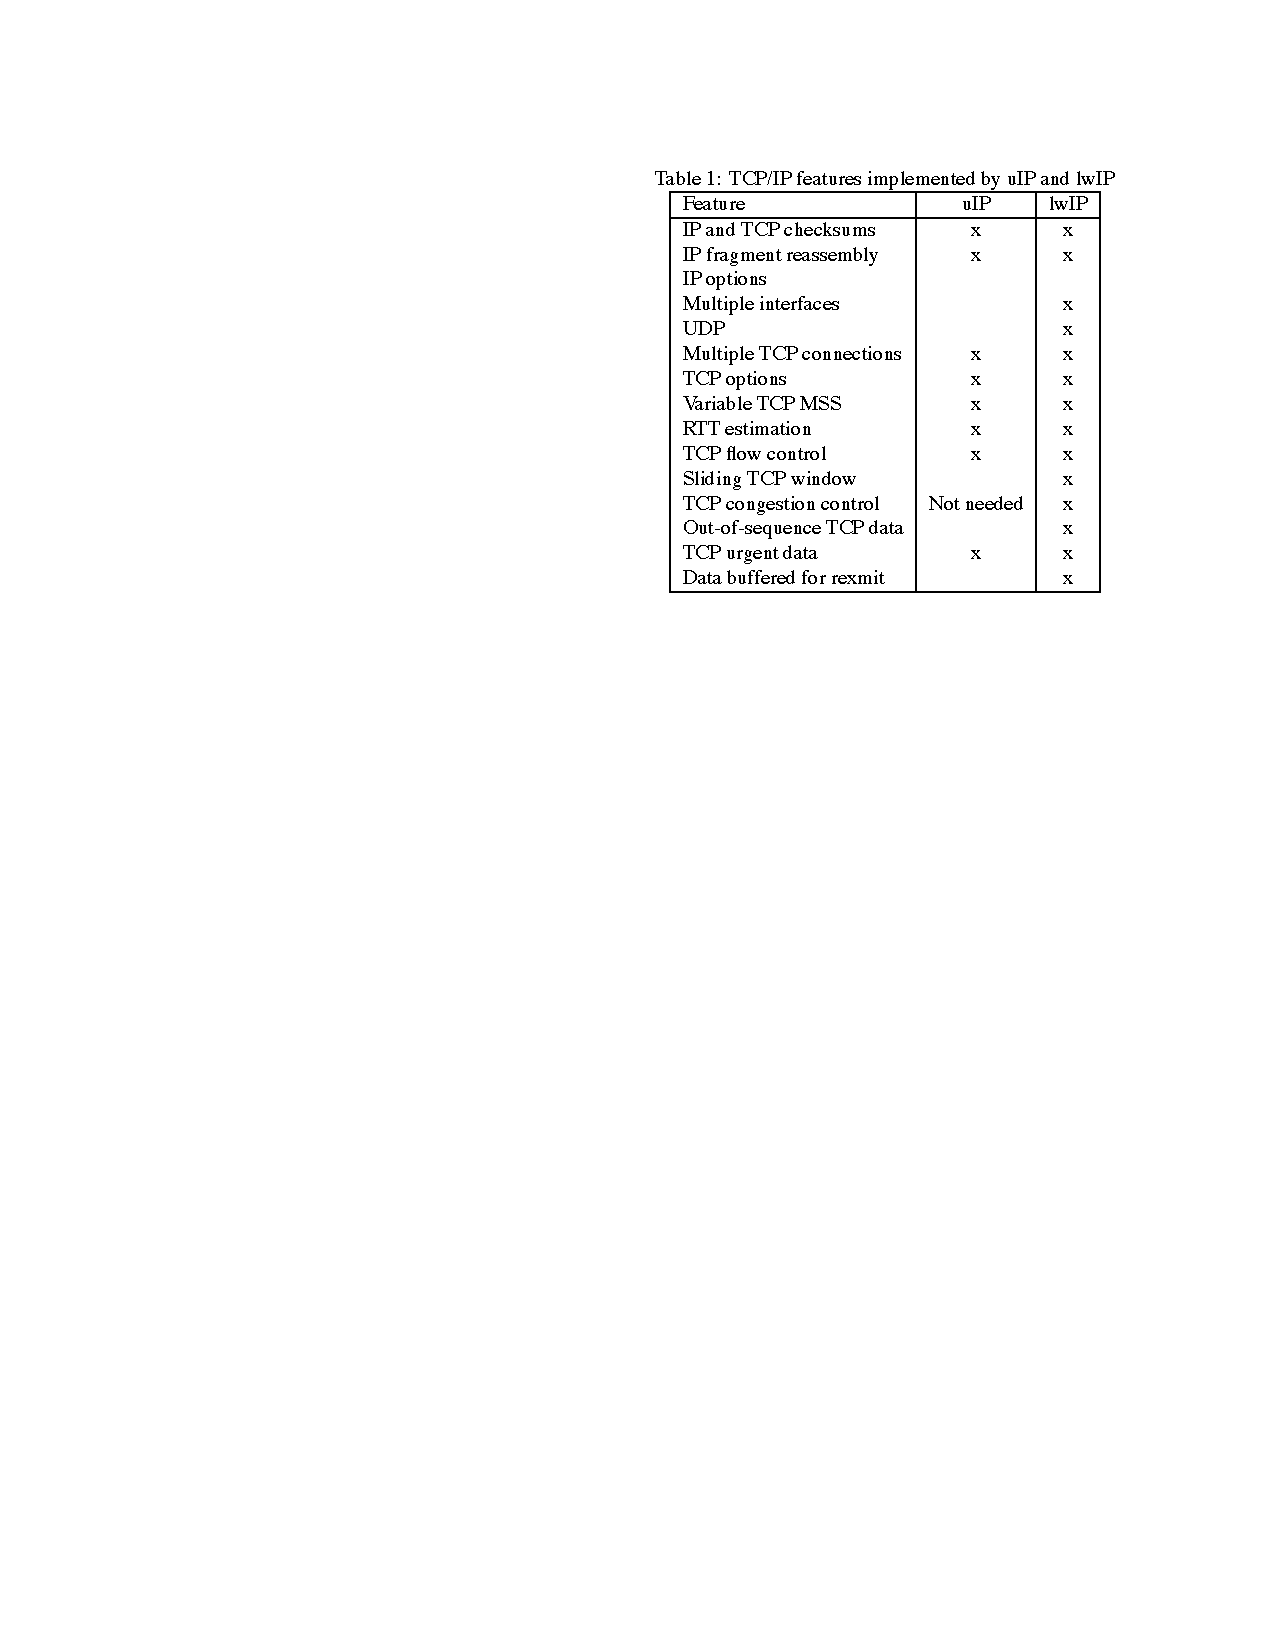
\includegraphics[width=.9\linewidth]{dunkels-uip-and-lwip}
      \caption{Features of $\mu$IP and the now no longer maintained lwIP. Since the table was published in \citep[p.4]{dunkels2003full} UDP has been added as well to $\mu$IP.}
      \label{fig:uip-features}
   \end{minipage}
\end{figure}

One important reason as to why $\mu$IP can achieve such a low memory footprint is that is liberates the OS from the complicated transmission of data between application and IP stack. Most of the requirements associated with this interface, as described in the RFC, are waived in \citep[p.4]{dunkels2003full}. This not only removes the need for a lot of software logic, but also allows a drastic simplification of transmission buffer management, something which its designer have used to the fullest extent: there is only enough buffer space for one packet at any time, including the need of transmissions as well as receptions. Figure \ref{fig:uip-ml} describes the main loop of $\mu$IP which explains its buffer management. The application that wish to transmit data copies it into $\mu$IP's buffer and then calls the transmission function with the appropriate addressing information. Upon reception, the procedure is the opposite. The stack figures out which application is interested in the arrived piece of data, then calls its handler, which in turn is programmed to react on the data and to produce a reply, which in turn is written to the very same buffer and so on.

Even though an IP packet can be well over a kilobyte in size (the MTU\footnote{Maximum Transmission Unit: The largest size of a packet that a network or a host can handle.} of IPv6 is 1280 bytes), the buffer can still be much smaller than this if used in conjunction with a MAC\footnote{Medium ACcess} layer that has a small MTU (6lowPAN (using IEEE 802.15.4 in turn) is very popular for Contiki and has a MAC MTU of at most 102 bytes\citep[section 4]{rfc4944}). This will allow the incoming IP-packet fragments to be spoon-fed to the receiving application, negating the need for a large buffer for transmission purposes. Buffer size then becomes a problem of how large IP-packets one wants the applications to transmit.

\section{Internet Security}
\paragraph{Security on the Internet} was, and is, as of today an unresolved issue in the author's opinion. As its protocol, IP, was originally designed and developed in the open world of academic computer science, no security considerations were made. Instead, the three properties of information security (confidentiality, authenticity, integrity) \citep[section 8.1]{vasseur10interconnecting} were provided by physically protecting the network hardware and the imposition of social norms among its users and operators. As the Internet grew, this and other weaknesses started to become problems. In 1995, the IETF\footnote{The Internet Engineering Task Force is the governing body of the development of Internet standards.} released a number of documents starting with RFC\footnote{RFC, or Request For Comment, is the collective name of the IETF's standards} 1883\cite{rfc1883} that defined IPv6, the planned successor of IPv4. IPsec was developed in conjunction with IPv6 and was until the advent of RFC 6434\cite{rfc6434} in late 2011 a mandatory part of a compliant IPv6 host. However, adaption of IPv6 has been slow despite growing technical problems with the still incumbent IPv4. The resistance to upgrade is widely attributed to the fact that the cost and risk (software adaption, operator training, equipment replacement etc) of making the change in most networks outweighs the potential benefits. This equation will certainly change, if slowly, in the coming years. In the meantime, IPv6 has found to be a great boon to new networks like Internet-connected smart phones, Internet-enabled set top TV-boxes and, naturally, the Internet of Things. In these cases it can be argued that the cost of adopting the legacy IPv4 is roughly the same as that of adopting IPv6, while enjoying benefits of the later's simplicity, auto configuration features and more\footnote{See chapter 15.1 in \cite{vasseur10interconnecting} for a brief discussion about the benefits of IPv6 over IPv4 in the context of IoT.}.

\paragraph{IPsec is a suite of protocols} that secures IP packets in an end-to-end fashion. Flows of packets, distinguished by properties such as source and target address, transport layer protocol, etc can be defined and different security policies applied. The system is not only limited to \emph{host-to-host} packet flows, but also allows a host to act as a gateway (termed \emph{security gateway} in the IPsec standard), enabling a secure link between two networks (\emph{network-to-network}) or a network to a host (\emph{network-to-host}). The suite can be implemented either directly in the IP stack of a host, but may also be located between the link layer and the network layer\citep[section 3.3]{rfc4301}, facilitating retrofits of existing stacks.

\begin{figure}[h!]
   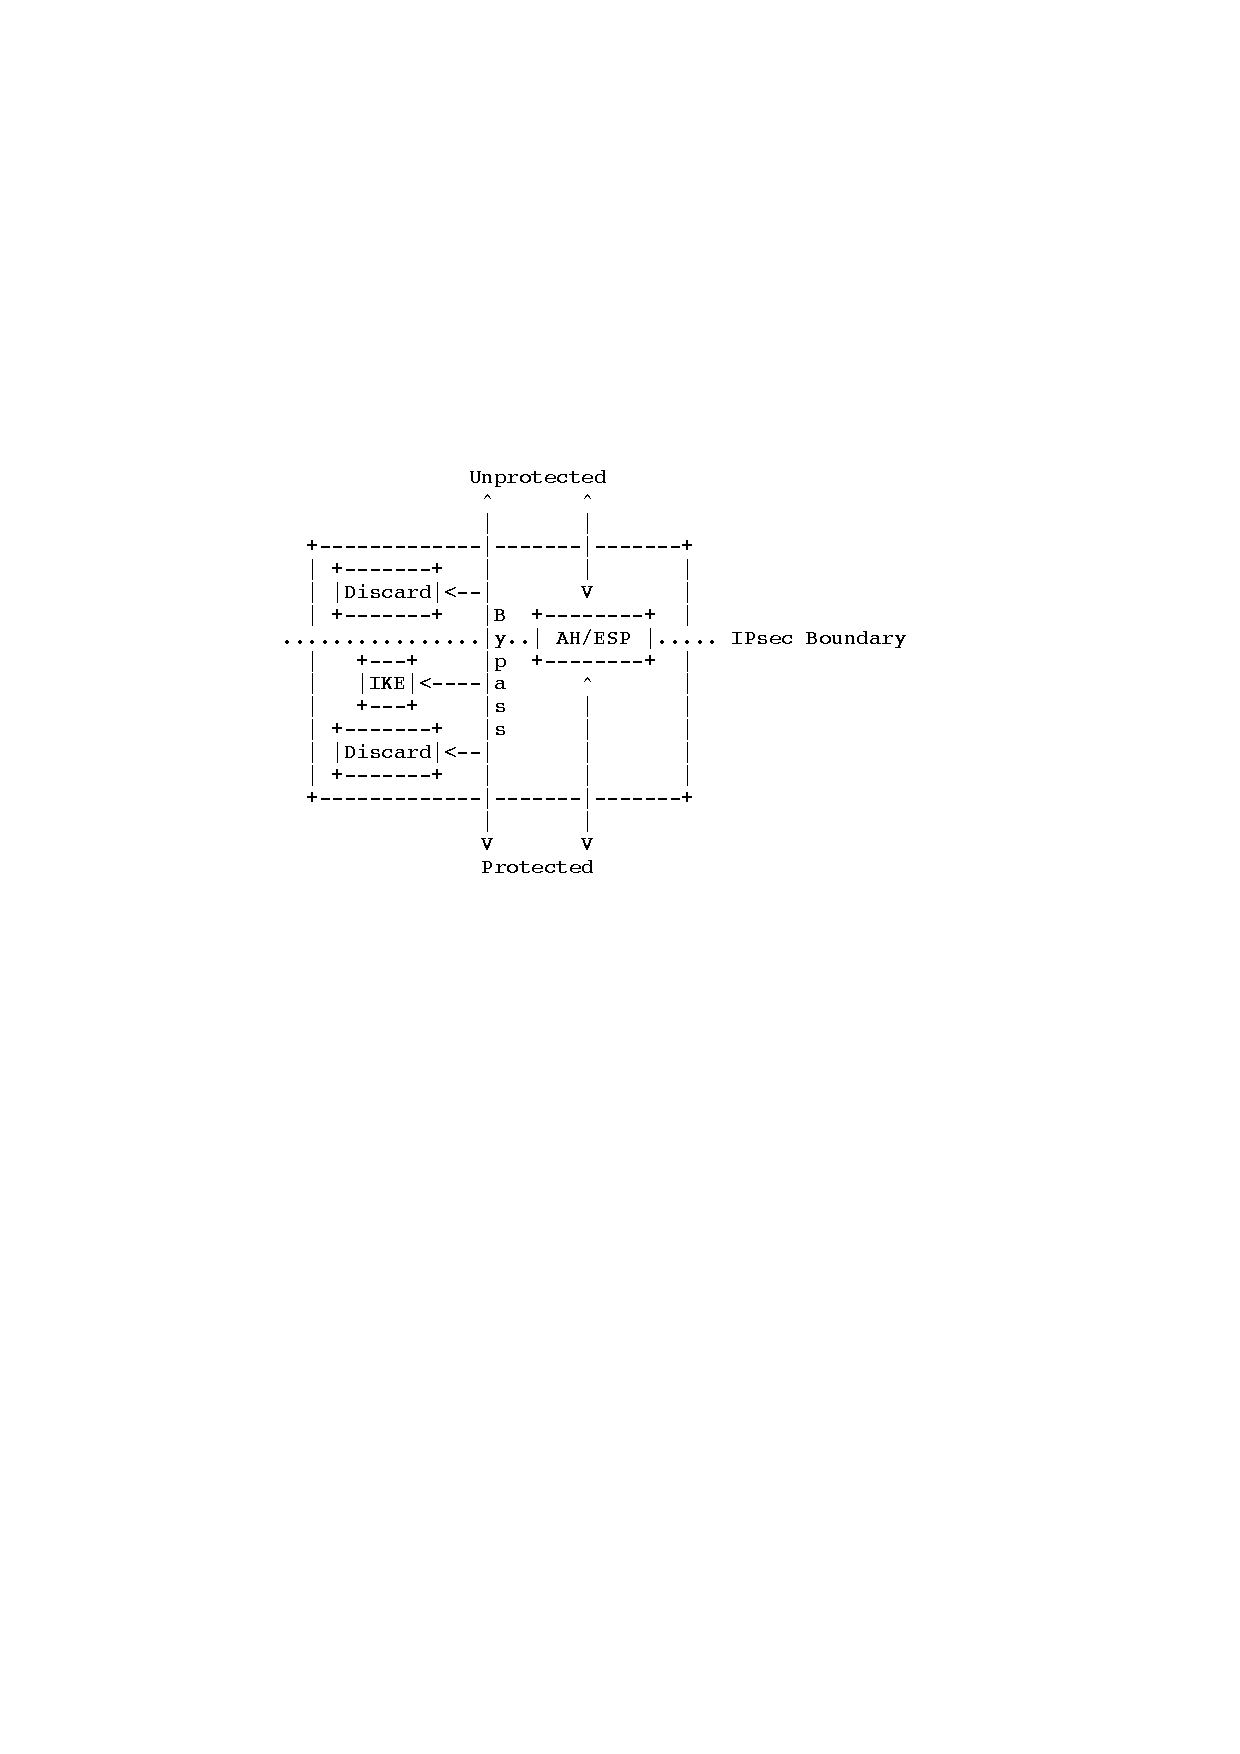
\includegraphics[width=0.9\textwidth]{ipsec-flow}
   \caption{IPsec processing of IP-packets. From \citep[p.8]{rfc4301}.}
   \label{fig:ipsec-flow}
\end{figure}

\label{ipsec_proc}
\paragraph{In the IPsec processing model} IP-packets are said to be passed between from \emph{protected} to \emph{unprotected} interfaces and vice versa. In the usual case, such as above, there are only one of each. The unprotected interface is always the interface connected to the insecure network, while the protected may be either connected to a secure network (the \emph{security gateway} configuration) or be attached to an operating system's IP stack (FIX: Is the last statement ok?). The flow of packets between the protected and unprotected interfaces are determined by policies set by the system administrator which are expressed in terms of network- and transport-layer primitives, i.e. IP addresses, port numbers and transport-layer protocols. The policy can cause a packet to be: thrown away (\emph{DISCARD}); forwarded over the IPsec boundary without any action taken (\emph{BYPASS}; removing or applying cryptographic protection of the packet (\emph{PROTECT}). The later is performed in the module named \emph{AH/ESP} in the fig. no. \ref{fig:ipsec-flow} which we will discuss in length further on (FIX: NO ref to place of disc.?).

\paragraph{A central concept} of the IPsec model is the data structure named the \emph{Security Association} (SA). A Security Association defines a single simplex IP link and the security services it provides to the traffic that it carries. The services can be implemented by one of the two IPsec protocols: \emph{Authentication Header} (AH) and \emph{Encapsulating Security Payload} ESP. Bi-directional (duplex) traffic is enabled by creating a pair of SAs, one for each direction. As the author will show, the SA is used by almost all IPsec components and we will return to it from time to time.

\paragraph{The policies and cryptographic secrets} used in IPsec processing are stored in three databases: the Security Association Database (\emph{SAD}); the Security Policy Database (\emph{SPD}) and its caches; the Peer Authorization Database (\emph{PAD}). The standard stresses the fact that the implementation of these databases should not be viewed as pre-requisites for a compliant IPsec implementation, but that such a system should exhibit the very same behavior as that of a system whose architecture was implemented in line with the standard's model. In the following paragraphs these databases will be used as constructs to explain the inner workings of IPsec, although, as the reader will learn in the \prettyref{cha:doi}, the author has actually used these constructs in the final implementation as well. Finally, the system will be explained only in brief as the IPsec suite is simply too large for a thorough review in this thesis. The interested reader is advised to read the complete standard document\citep{rfc4301} starting at section 4.4 for an in-depth definition of the SAD, SPD and PAD.


\paragraph{The SPD} stores the policies that controls IPsec processing. It consists of an ordered list, where each entry is composed of a set of \emph{selectors}, \emph{PFP flags} and a \emph{processing action}. 

The \emph{selector} is a data structure that represents a traffic pattern between hosts or networks and serves to distinguish what traffic the policy in question is referring to. The fields are as follows: Local address; Remote address; Next Layer Protocol (e.g. TCP, UDP, ICMP); Local Port (This is dependent upon protocol type, e.g. in the case of an ICMP packet message type and code is listed instead.); Remote Port. Full specifications are found in \citep[Section 4.4.1.1]{rfc4301}.

PFP, or \emph{Populate From Packet} flags, are rules used in conjunction with the instantiation of an SA on the basis of the SPD entry. Instantiation in this context means that the newly created SA's selector (which has a similar purpose to a SPD entry's selector) is completed with information from that of the SPD entry's selector. However, for each of the selector's fields there is a corresponding PFP flag. If that flag is set, that field will be populated with information from the packet that triggered the instantiation. This process will be explained in detail further on as it's a central mechanism.

The \emph{processing actions} are the very same as described in \ref{ipsec_proc}: \emph{DISCARD}; \emph{BYPASS}; \emph{PROTECT}. The action \emph{PROTECT} differs from the the other actions in the sense that is also includes settings of how to protect the traffic, e.g. using a security gateway (tunneling), DSCP\footnote{Differentiated Services Code Point; QoS for IPv6} services, various SA settings used in instantiation.

\paragraph{The SPD's caches} can be divided into three different sections: SPD-O outbound traffic that is not to be protected; SPD-S for outbound traffic that is to be protected; SPD-I for all incoming traffic. The entries contains the same fields as the SPD, with the exception of the PFP (`Populate From Packet', as described above) field which is not present. From a functional point of view, each entry is an \emph{instantiation} of an SPD entry. That implies that each entry's selector is a subset of one of the SPD's entry's selectors. The IPsec processing mechanism creates such entries in response to encountering traffic that uses one of the SPD's entries. This is made because of two reasons: 

\begin{quotation}
1) Lookups in the SPD can be slow on large systems with many SPD entries. The SPD cache is faster\footnote{As to the question of why the SPD's cache allows a faster lookup, the author has to direct the reader to RFC 4301. This speedup is hardly relevant to the thesis in question and thus the curious reader is encouraged to start reading at section 5, taking extra care to read the parts about de-correlation.}.
\end{quotation}

\begin{quotation}
2) a rule in the SPD can order traffic for a large address space to be protected. That address-space can contain many hosts, and each host can in turn demand different SAs for different traffic (e.g. different SAs for traffic over TCP and UDP). Thus, one realizes that each SA must explicitly define what traffic it carries. This is one of the purposes of the SPD-S cache. Each entry corresponds to an SA and its selector defines its traffic.
\end{quotation}

It's unfortunately hard to get a good overview of the SPD's caching system as the information is sprinkled over large parts of RFC 4301. The author recommends the curious reader to begin reading at section 5, `IP traffic processing'\citep[Section 5]{rfc4301}.



% SPD-S outbound prot. traffic: Selectors and more goes here for instansiated SAs
% SPD-O outbound nonprot. traffic: fast lookups
% SPD-I inbound nonprot traffic: fast lookups

%There is nominally one cache per SPD.

% The IPsec implementation context determines how selectors are used. For example, a native host implementation typically makes use of a socket interface. When a new connection is established, the SPD can be consulted and an SA bound to the socket. Thus, traffic sent via that socket need not result in additional lookups to the SPD (SPD-O and SPD-S) cache. In contrast, a BITS, BITW, or security gateway implementation needs to look at each packet and perform an SPD-O/SPD-S cache lookup based on the selectors.

\paragraph{The SAD} stores the IPsec system's \emph{Security Associations} (SAs). The purpose of the database is to store the parameters of the system's SAs, but can be used to store other information as well. RFC 4301 outlines in section 4.4.2.1 fifteen required fields and because of space constraints, this section will only list the ones deemed most important by the author.

Security Parameter Index (SPI): Each SA is identified by a 32-bit value. This value is selected by the receiving end of an SA to be unique. This makes it possible for a system to uniquely associate inbound traffic with an SA using the SPI number as the key. Outbound traffic processing uses the SPI number to construct the IPsec headers.

Sequence Number Counter: Every IPsec system maintains a counter for each SA that is incremented by one for each packet that it carries. This information is used in IPsec packet processing and anti-replay protection (as will be explained below.)

Anti-Replay Window: A counter and a bit-map used for detecting packets that have been replayed by an attacker\footnote{In a replay attack, a packet is intercepted by a man-in-the-middle with the purpose of delaying or repeating it. This can trick the targeted system into revealing secret information e.g. reusing the same keys in a stream cipher.}. The anti-reply protection is available for the AH as well as the ESP security protocols, but only when using automatic key management (more on this later).

Symmetric encryption information: Encryption algorithm and IPsec protocol type (AH or ESP) used by the SA along with necessary secrets (keys etc) and parameters.

SA Lifetime: A limit at which the SA should be terminated, expressed in either time or the number of bytes transported by the SA.

%each containing the parameters of , each consisting of the following substructures: a \emph{selector}, and an \emph{action}.


\paragraph{The PAD} (section 4.4.3) is controlled by the administrator and used by the security association management protocol along with the SPD to negotiate new SAs. The core purpose of the database is to store 1) the identification tokens of the peers that the system is allowed to communicate with and 2) the authentication mechanism, parameters and data of each aforementioned peer.


% stores the authentication requirements for 5. As SAs can be created both manually by an administrator as well as automatically by a Key Exchange service such as IKE, 

%Security policies are stored in in the \emph{Security Policy Database} (SPD). It consists of several entries, each consisting of the following fields: a \emph{selector} that defines a certain traffic flow; . The selector includes source address range, destination address) by means of \emph{}
% 
%  are said to be members of a communication session for which the same security policies are applied. Such sessions can be   that can be implemented directly in the IP stack of a host or in a router 

% \paragraph{IPsec's security model} differs from that of the one commonly used by security protocols operating in the higher layers e.g. TLS and SSH. Instead of using primitives such as user identity or tickets to create secure connections or make policies, IPsec  uses the concept know to IP such as hosts, networks and upper layer protocols such as TCP or UDP.  and .. primitives known to IP; ports, transport layer protocols, networks and host IP-addresses. 
% 
% host-to-host
% network-to-network
% SAD
% SPD


\section{Understanding the IP headers} are key to understanding IPsec. The author will therefore quickly review the structure of the IPv6 headers before moving on to explain their relationship to IPsec. Below the readers finds a schematic of the IPv6 header, also called the IPv6 `fixed header' for reasons that soon are to be discussed.

\begin{figure}[here]
   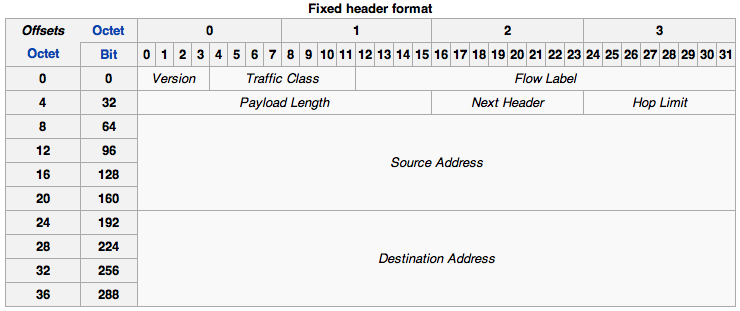
\includegraphics[width=0.9\textwidth]{wiki-ipv6-header}
   \caption{The IPv6 header. Figure from \cite{wiki:ipv6_packet}.}
   \label{fig:ipv6_packet}
\end{figure}

As the author assumes that the reader is acquainted with the general principles of IP networking, the discussion of the above header fields will be brief. \emph{Version} is always six; \emph{Traffic Class} (reminiscent of the IPv4 \emph{TOS} field) and \emph{Flow Label} are for flow and congestion control, which are of no concern to us; \emph{Payload Length} is the length of the payload field, including any so called `extension header' (more on this soon); \emph{Next Header} specifies the packet's transport layer protocol, or the first extension header's type if one is present; \emph{Hop Limit} is equivalent to IPv4's Time-To-Live field which is decremented by each router along its path, ultimately to be discarded when it reaches zero.

IPv4 placed all of its settings into one big header, many settings which as of today are rarely used, and the possibility of extending it with new features are severely limited. The designers of IPv6 solved this problem by keeping the fixed header (figure \ref{fig:ipv6_packet}) small and allowing it to be extended by a mechanism called \emph{extension headers}. The extension headers contain any optional information, information which can be intended for the packet's destination host and/or intermediate routers along its path. Although the information is usually supplied by the source host, some headers (such as \emph{Fragment}) can be altered and/or added by routers.

\begin{figure}[here]
   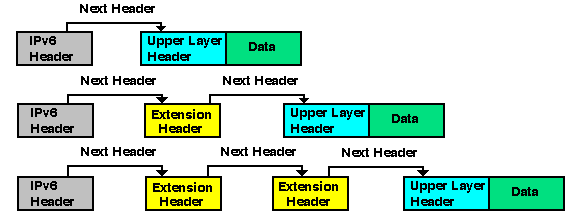
\includegraphics[width=0.9\textwidth]{ipv6-nextheader}
   \caption{Illustration of IPv6's next header scheme. FIX! Not received permission! Source:http://www.zytrax.com/tech/protocols/ipv6.html}
   \label{fig:ipv6_nextheader}
\end{figure}

\begin{figure}[here]
   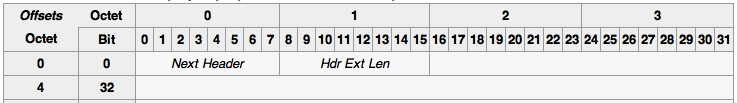
\includegraphics[width=0.9\textwidth]{wiki-ipv6-nextheader}
   \caption{The generic mandatory part of an `extension header'. Figure from \cite{wiki:ipv6_packet}.}
   \label{fig:wiki-ipv6-nextheader}
\end{figure}

The extension header scheme is basically a linked list (figure \ref{fig:wiki-ipv6-nextheader}). The field \emph{Next Header} denotes the type of extension header to come or, if this is the last extension header, the packet's type of transport layer; \emph{Hdr Ext Len} is the length of this extension header in multiples of eight octets, not including the first eight octets. The rest of the next header contains data that is specific to each next header type.

\begin{figure}[h!]
   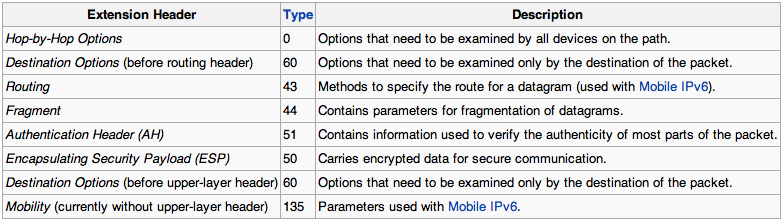
\includegraphics[width=0.9\textwidth]{wiki-ipv6-listofextensionheaders}
   \caption{This list covers a number of common extensions headers `next header'. List from \cite{wiki:ipv6_packet}.}
   \label{fig:wiki-ipv6-listofextensionheaders}
\end{figure}


\section{The AH protocol in IPv6}
\begin{figure}[h!]
   % 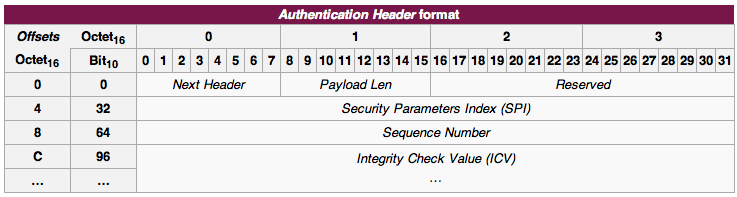
\includegraphics[width=0.9\textwidth]{wiki-ipsec-ah}
   % \caption{The AH extension header. From \cite{wiki:ah_header}.}
   % \label{fig:wiki-ipsec-ah}

   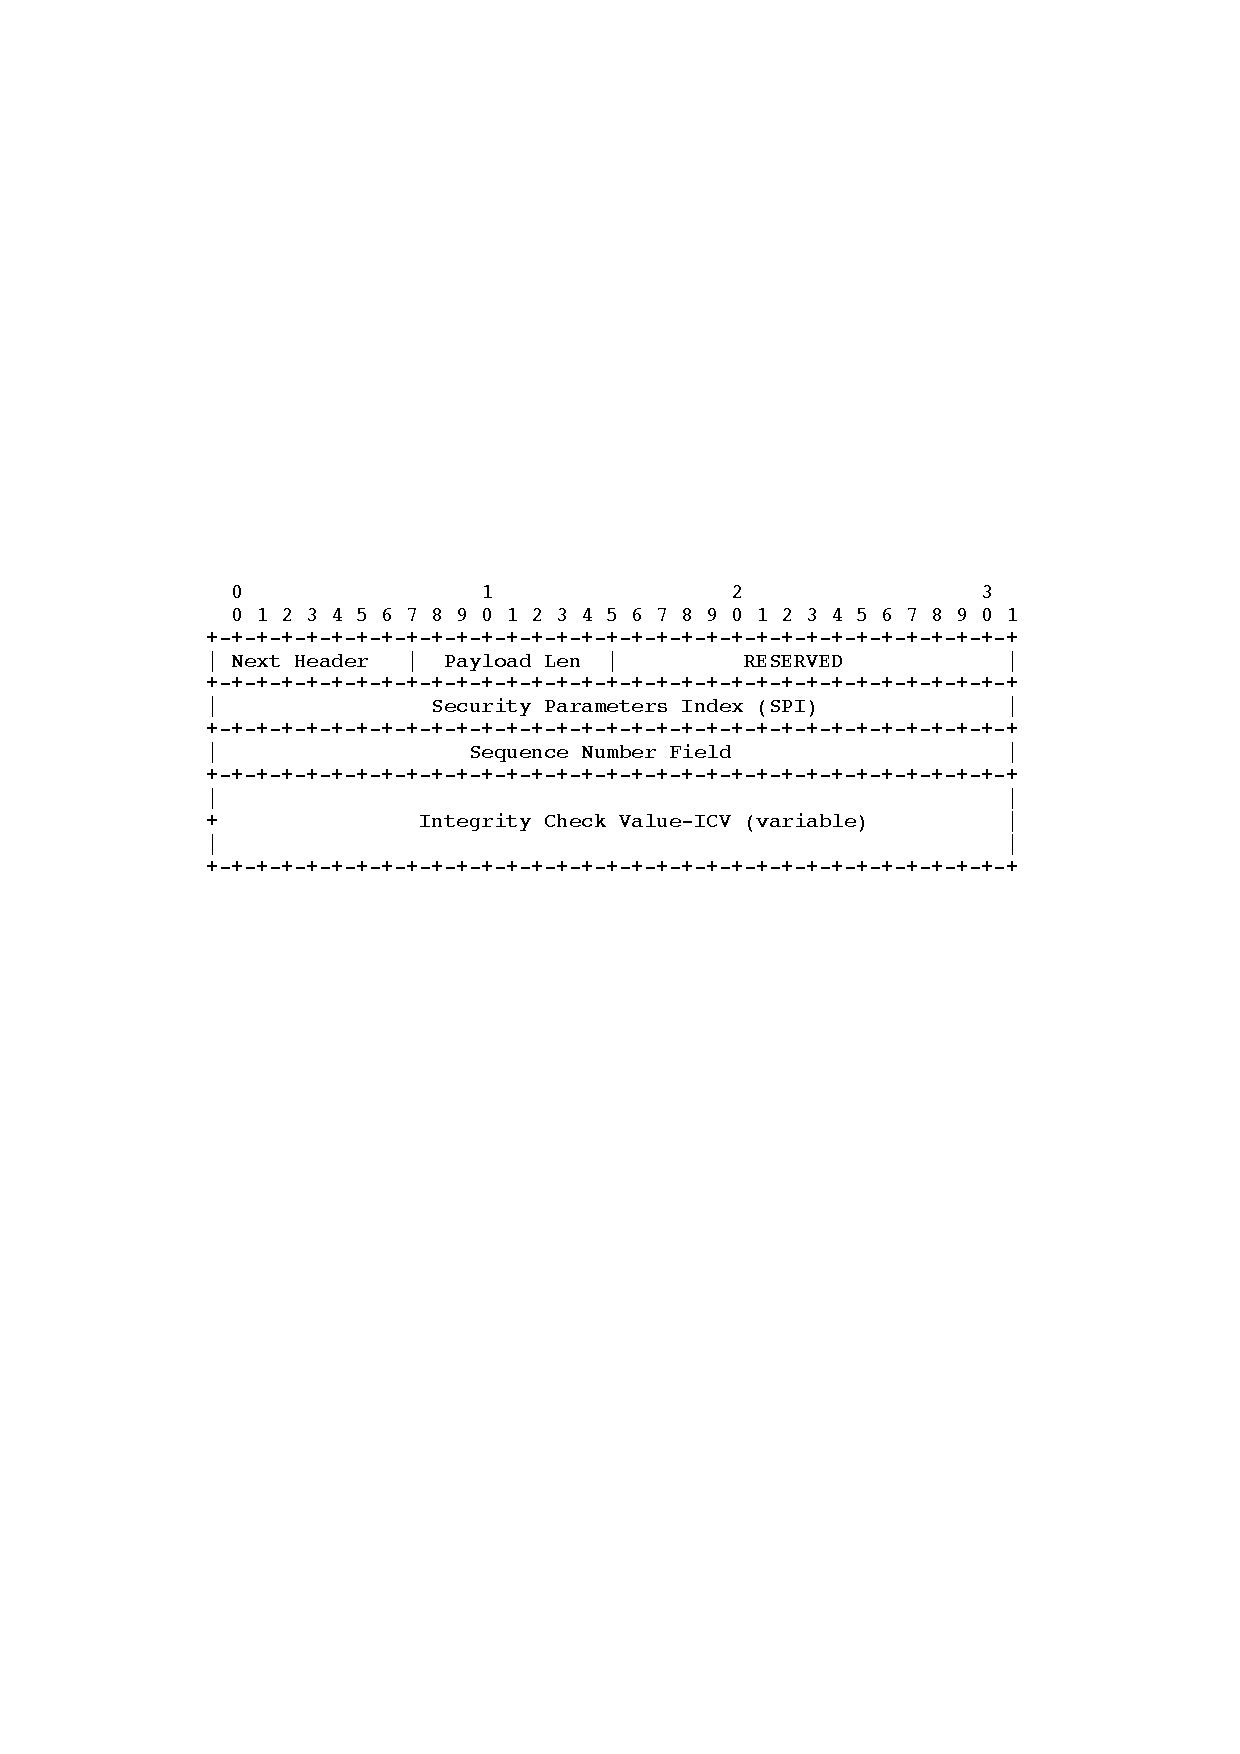
\includegraphics[width=0.9\textwidth]{ah_nextheader}
   \caption{The AH extension header. From \cite{rfc4302}.}
   \label{fig:wiki-ipsec-ah}

\end{figure}

The AH protocol's header (\emph{Authentication Header}) protocol described in RFC 4302\cite{rfc4302} guarantees the \emph{data integrity} and the \emph{data authentication} (origin) of the IP packet which it is applied to. This is achieved by applying a \emph{Message Authentication Code} (MAC) to the packet's content and to the header's immutable fields using a key privy to the two parties.

\begin{figure}[h!]
   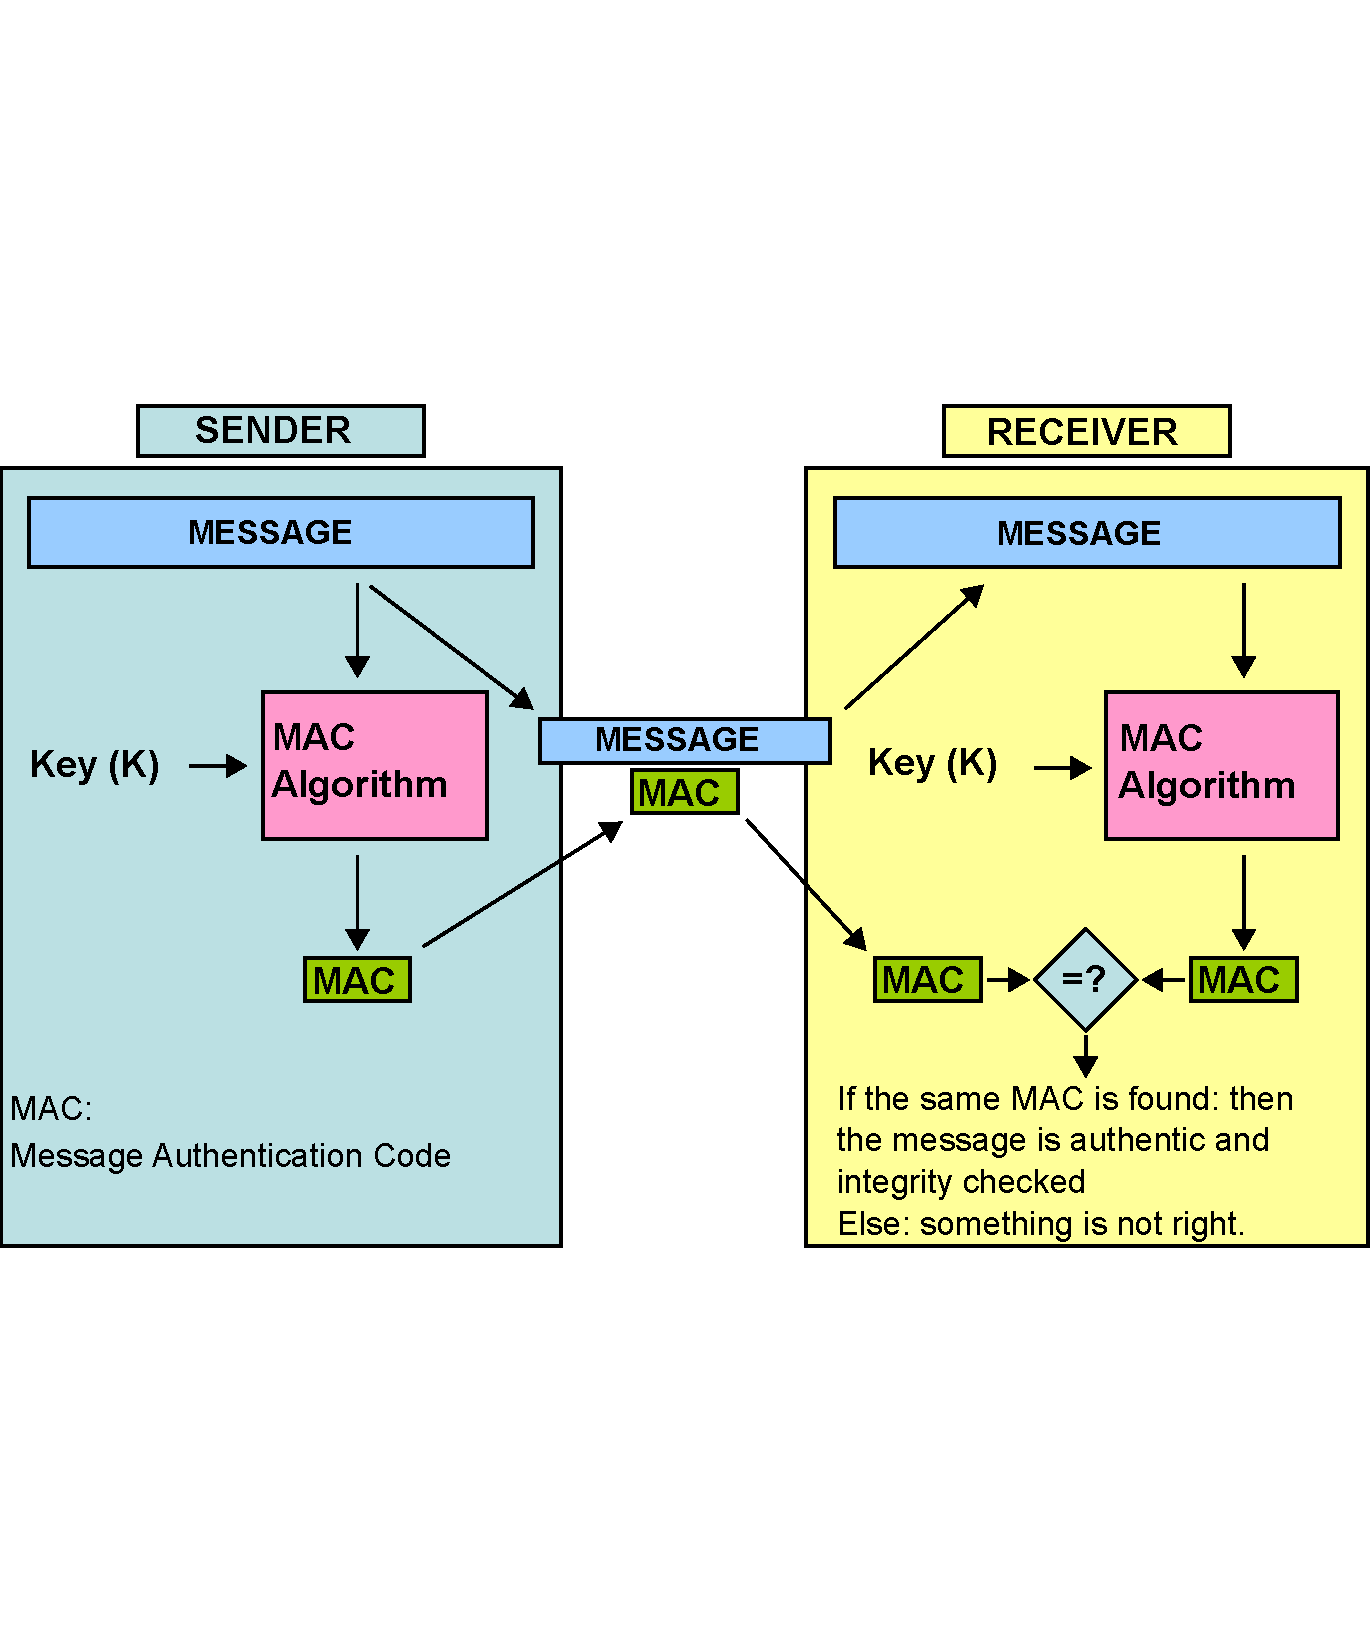
\includegraphics[width=0.9\textwidth, trim=0 205 0 210]{wiki-mac}
   \caption{Message Authentication Code. From \cite{wiki:mac}.}
   \label{fig:wiki-mac}
\end{figure}

Figure \ref{fig:wiki-mac} describes the principles of a MAC algorithm: The message, composed of the packet's payload and its immutable fields, are combined and digested\footnote{A synonym of \emph{digested} is \emph{hashed}.} along with a key. This produces a \emph{MAC} string (also referred to as a \emph{digest} or \emph{hash} string) which is attached along with the message. IPsec refers to this value as the \emph{ICV}.

Upon arrival the receiver performs the same calculations and compares the resulting \emph{MAC} with that included in the packet. This scheme will, if correctly implemented and algorithms chosen with care, make it computational infeasible\footnote{A security attack is said to be `Computationally Infeasible' if the required cost of performing the necessary cryptographic computations are outside the reach of even very large organizations.} for an attacker to alter the message without knowledge of the key. As a side benefit, the packet is also protected against accidental corruption such as transmission errors.

The parameters of the process (such as key, key length and type of MAC algorithm) are SA-specific and are stored in its data structure.




\section{The ESP protocol in IPv6}

\begin{figure}[h!]
   % 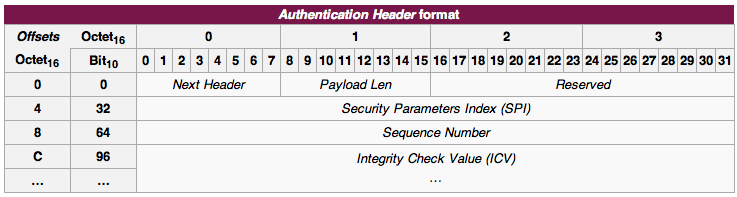
\includegraphics[width=0.9\textwidth]{wiki-ipsec-ah}
   % \caption{The AH extension header. From \cite{wiki:ah_header}.}
   % \label{fig:wiki-ipsec-ah}

   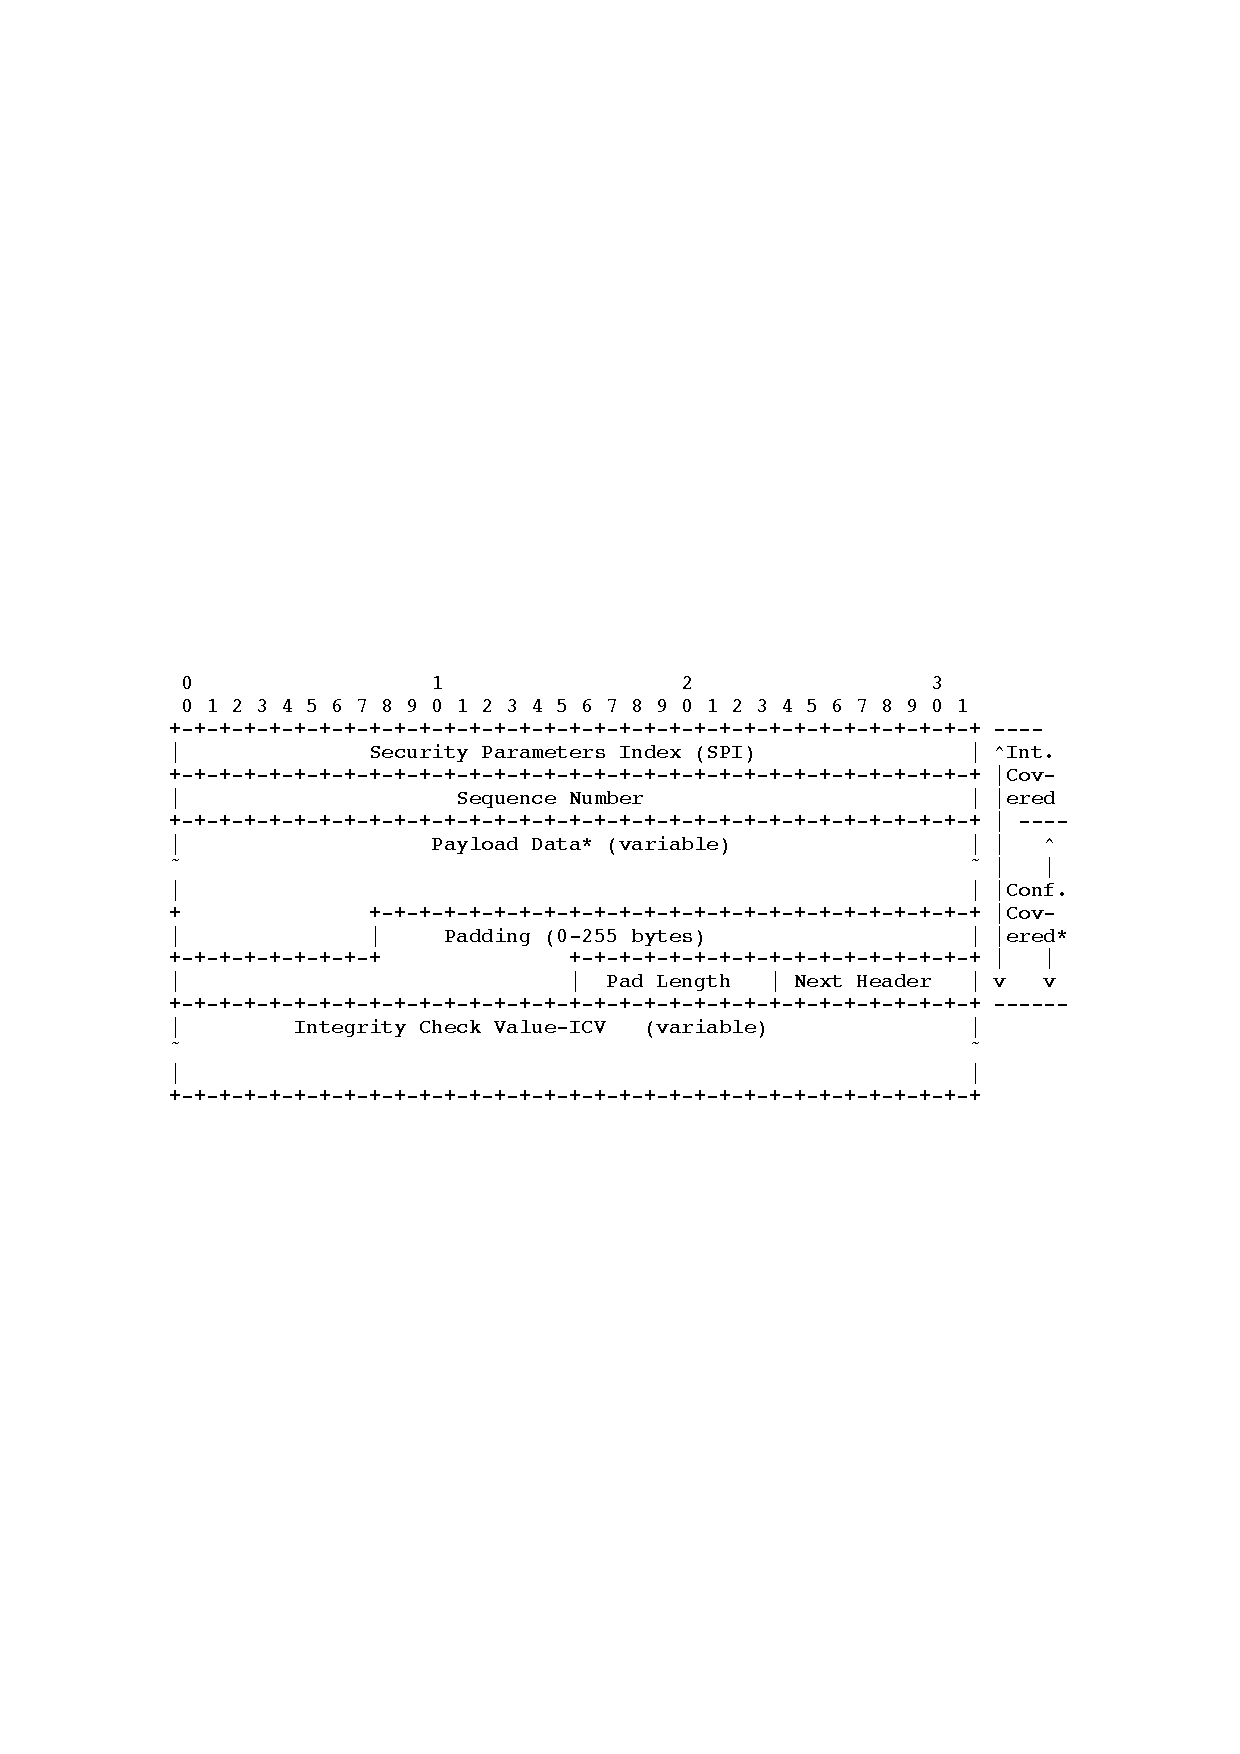
\includegraphics[width=0.9\textwidth]{esp_nextheader}
   \caption{The ESP IPv6 extension header. From \cite{rfc4303}.}
   \label{fig:wiki-ipsec-esp}
\end{figure}

The ESP (Encapsulating Security Payload) protocol described in RFC 4303\cite{rfc4303}, provides \emph{confidentiality} and limited \emph{traffic flow confidentiality} in addition to AH's \emph{data integrity} and \emph{data authentication}. The term \emph{Encapsulating} is derived from the fact that the protocol is designed to encase everything that follows it in the packet (extension headers as well as payload). This practice is of benefit in itself, but rather it facilitates the implementation of confidentiality protection. For example, there are many popular algorithms which belongs to the block cipher family e.g. AES-CBC. Such algorithms only operates upon fixed sizes of data and therefore needs to pad\footnote{To `pad' data is to prepend or append white space characters (in the case of text documents) or null bytes to a string in order to increase it to a predetermined length.} the IP packet's payload to a multiple of the block length.

The fact that confidentiality protection is optional makes ESP services identical to that of AH's, but only under certain circumstances. In \prettyref{cha:doi} it will be shown how this fact can be exploited.


% \cite{wiki:ipv6_packet}
% 
%  architecture has always been open
% * Protects everything from the network level and up (Model)
% * Symmetric encryption
% * Security associations
% 


\section{Automatic key management (IKEv2)}%{Automatic negotiation of SAs (IKEv2)}
We have now explained the essentials of IPsec: the databases and their relations to each other and how they govern the flow of packets in the IPsec stack. This functionality is all that is required for an interoperable IPsec implementation. However, this requires all SAs to be set by the administrators of the systems in question. I.e. if two such hosts wants to communicate by IPsec the administrators must agree upon, and manually create, the SAs along with their encryption keys and associated settings. Naturally, we would like to automate this in order to lessen the human's workload. This is the purpose of an IPsec Key Management Protocol. At of the time of this document's writing, there are several protocols: IKE (defined in RFC 2407 - 2409)\cite{rfc2407}\cite{rfc2408}\cite{rfc2409}; IKEv2 (RFC 5996)\cite{rfc5996}; KINK (RFC 4330)\cite{rfc4330} and IPSECKEY (RFC 4025)\cite{rfc4025}. What they all have in common is that they solve the problem of automated key management, albeit in different ways, and that they all interface with IPsec through its databases.

However, this thesis will henceforth only discuss IKEv2 as it's the de-facto standard and, more importantly, the original target of study for this thesis. IKEv2 is the successor to IKE that was widely regarded to be a standard that suffered from unnecessarily complicated and vague standards documents. This issues were addressed in IKEv2 and resulted in, most importantly: better interoperability among implementations; faster keying handshake; less complex codebase.

\subsection{Overview}
As previously stated, IKEv2 is a component that is wholly external to the parts that we have covered so far (IPsec packet processing, SPD, SAD etc). The former are usually, in a general purpose operating system, implemented in the kernel\footnote{Linux's current IPsec implementation follows this model, and the author believes Microsoft's equivalent for Windows does so as well.} while the latter is written as service running in user space. This is the preferred method on an IPsec host as IPsec's packet processing mechanism needs to be implemented in conjunction with the OS' network stack (referred to as `bump-in-the-stack' or `native' in RFC 4301\citep[p.10-11]{rfc4301}) while IKEv2 is shaped into a user-space service. Naturally, we want as much code as possible to run in user space as it facilitates development and allows better integration with the rest of the operating system.

\subsection{Negotiating SAs}
IKEv2 communicates with other IKEv2 capable hosts by means of UDP datagrams on port 500. As the purpose of the communication is to negotiate new SAs, the communication can not be protected by any IPsec SAs. Therefore, a correctly configured IPsec host must allow non-protected traffic on this UDP port. In this section we will explain how IKEv2 itself creates a secure communication channel for its datagrams. This begins with the following exchange of data, as described in IKEv2 standards document, RFC 5996\citep[p.5]{rfc5996}:  


\begin{quotation}
All IKE communications consist of pairs of messages: a request and a response. The pair is called an `exchange', and is sometimes called a `request/response pair'. The first exchange of messages establishing an IKE SA are called the IKE\_SA\_INIT and IKE\_AUTH exchanges; subsequent IKE exchanges are called the CREATE\_CHILD\_SA or INFORMATIONAL exchanges. In the common case, there is a single IKE\_SA\_INIT exchange and a single IKE\_AUTH exchange (a total of four messages) to establish the IKE SA and the first Child SA. In exceptional cases, there may be more than one of each of these exchanges. In all cases, before any other exchange all IKE\_SA\_INIT exchanges MUST complete type, then all IKE\_AUTH exchanges MUST complete, and following that, any number of CREATE\_CHILD\_SA and INFORMATIONAL exchanges may occur in any order. In some scenarios, only a single Child SA is needed between the IPsec endpoints, and therefore there would be no additional exchanges. Subsequent exchanges MAY be used to establish additional Child SAs between the same authenticated pair of endpoints and to perform housekeeping functions.
\end{quotation}

The `IKE SA' referred to in the above text is an type of SA that is only for IKE communication. It is not used by the IPsec processing system, but only by the IKE service to secure its communication with other hosts. The creation of the `Child SA' is the final goal of the IKE connection - an SA to be used by the IPsec system to protect some part of the host's traffic. Its name can be derived from the fact that its cryptographic material is based upon that of the IKE SA's i.e. it can be said to be a descendent. On the next page (no. 6), the standard continues by providing more details about the SA negotiation:

\begin{quotation}
The first exchange of an IKE session, IKE\_SA\_INIT, negotiates security parameters for the IKE SA, sends nonces, and sends Diffie- Hellman values. The second exchange, IKE\_AUTH, transmits identities, proves knowledge of the secrets corresponding to the two identities, and sets up an SA for the first (and often only) AH or ESP Child SA (unless there is failure setting up the AH or ESP Child SA, in which case the IKE SA is still established without the Child SA). The types of subsequent exchanges are CREATE\_CHILD\_SA (which creates a Child SA) and INFORMATIONAL (which deletes an SA, reports error conditions, or does other housekeeping). Every request requires a response. An INFORMATIONAL request with no payloads (other than the empty Encrypted payload required by the syntax) is commonly used as a check for liveness. These subsequent exchanges cannot be used until the initial exchanges have completed.
\end{quotation}

As UDP is an unreliable transport layer, IKEv2 includes a mechanism for retransmission:

\begin{quotation}
An IKE message flow always consists of a request followed by a response. It is the responsibility of the requester to ensure reliability. If the response is not received within a timeout interval, the requester needs to retransmit the request (or abandon the connection).
\end{quotation}

After the handshake is complete (i.e. the creation of the SA for the IPsec traffic), the IKE SA is retained for future use as this will negate the need to re-create it whenever child SAs shared with that particular host need to be created or destroyed.


%FSM diagram of a handshake??


% \subsection{Interfaces}
% (PICTURE) IPsec processing, SPD, SAD, PAD <-> IKEv2
% 
% As stated earlier, IKEv2 communicates with IPsec by manipulating its databases. However, what has not been mentioned is that the IPsec processing system can signal IKEv2 as well. One such case is when the need for a new SA arises. Consider the following scenario:
% 
% \begin{quotation}
% An application on the host sends data destined for another host. When the resulting packet is received by the IPsec processing mechanism it tries to determine wether or not the packet is to be protected by trying to match its destination address with the selectors found in the SPD and its caches. If found in SPD and req. prot. invoke IKE.
% 
%\end{quotation}

%The same procedure occurs upon SA expiration: expiration of an SA in the SAD causes IPsec to signal IKEv2 that it needs to negotiate a new one.


% \subsection{Putting it all together}
% Final review of IPsec processing mechanism

% SKRIV-ANTECKNINGAR
% 0715: Måste säga något om tunnlar. Vart lägger jag det?


% * Handshakes for IPsec
% * Establishing security associations
% * Asymmetric encryption



\chapter{Design and Implementation}
\label{cha:doi}
Implementing Internet standards in Contiki is often a challenging task. Internet standards are written with the presumption of hosts with vastly more capable hardware on the host's part. This requires the engineer to simplify parts of the standard, make generalizations, and omit parts altogether. This might be difficult as it requires good knowledge of the standard in question as well as the behavior of other implementations. The synthesis of this knowledge allows her to save hardware resources by making shortcuts in her implementation, shortcuts which might very well violate the standard document, but still exhibit a behavior which allows communication with the rest of the Internet. This a good example of the very practical, experimental, approach that is typical of Contiki's development culture.

\section{Development process}
The original goal of this thesis was to develop a working IKEv2 implementation on top of of an existing IPsec implementation already developed for Contiki. Therefore the literature review started with the RFCs\footnote{Described in so the so called RFC (Request for Comments) publication managed by the IETF and the Internet Society} covering that standard, continuing with other documents as the author's understanding of the field grew. 

The author found the body of standard documents to be large, complex and described many features. It was unclear what effects a removal or alteration of a behavior could have on the implementation. Therefore the following principle was decided upon:

\begin{quotation}
\emph{The guiding design principle of the implementation} is that is must be a subset of the standard and follow the described architecture as close as possible. Any deviation from this requires a thorough analysis of the security implications or the implementation will lose its greatest benefit - the security properties brought by the thoroughly vetted IPsec standard.
\end{quotation}

Obviously, a thorough investigation and rework of the standards' internals would have the possibility of resulting in a more efficient implementation, but such an endeavor would require an effort that certainly would be outside the bounds of this work. 

Simultaneously, the author worked with Contiki's source code and documentation in order to figure out how to integrate IKEv2 and the IPsec system into Contiki, a feat easier said than done as Contiki is quite different from the typical multi-user multi-tasking operating system. Implementation then proceeded in a top-down fashion where the data structures were written first, APIs secondly and then finally the actual algorithms.

Contiki targets\footnote{A compiler is said to be \emph{targetting} a certain CPU's instruction set in the sense that it is configured to produce compatible binaries.} many different platforms, and two of them is Windows and Linux, i.e. the platform that the compiler is running on. This is called the \emph{native} target and is particular in the sense that Contiki (which is running as an ordinary process in the host's operating system) has access to the wast resources of the personal computer. Needless to say, this greatly facilitates debugging and was therefore used as the predominant build target during the development process. Peripherals such as sensors are emulated and network communication is achieved using a faked serial interface over a tunnel FIX:Look this up. 

\paragraph{During final development} the target was changed from \emph{native} to \emph{msp430} (a CPU commonly used in IoT platforms due to its energy efficiency) as the focus turned from functionality to memory and speed improvements. Benchmarking and tuning has to be performed on the correct platform as libraries, the platform's instruction set, and compiler optimization possibilities are target specific. Instead of using actual hardware\footnote{Using real hardware for testing purposes turned out to be a large problem as no readily available platform had the required memory capacity to store the binaries.} Contiki was executed on emulated hardware using Contiki's popular simulation environment - Cooja\cite{osterlind06crosslevel}. Apart from providing emulation, Cooja features a complete experimental sandbox which will be further described in the chapter Evaluation.


% As the author only had a rudimentary knowledge (roughly comparable as that of system administrator) of IPsec / IKEv2, he decided to that the safest way.

\section{IPsec}
At the project's inception, there was already a rudimentary implementation of IPsec in place (described in \cite{raza12secure}). It had the ability to receive as well as transmit AH as well as ESP headers, but could only handle one set of security parameters, effectively limiting the host to one SA that was used in a bidirectional manner. This did not scale and the natural idea was to go ahead and implement IKEv2 as well.

The author decided from early on to implement a subset of RFC 4301 and associated documents. This was done in order to comply with the \emph{design principle} as outlined earlier, but mostly so because the databases are good at what they do: the implementation can use the SAD to store the SAs; the processing mechanism can use the SPD for policy management etc. There are good reasons as to why theses entities were invented, and leaving them for something else would make the other parts of the system (i.e. IKEv2) harder to implement as the developer would be forced to invent new solutions for doing without these systems. That would increase the work burden as well.

\subsection{The IP processing mechanism}

We implement IPsec by inserting hooks into  the uIP-stack.


\subsection{The databases: SAD; SPD and PAD}
IPsec and IKE communicates through the databases SPD and SAD. The PAD doesn't need to be a database.



The IPsec subsystem is implemented inside the uIP6 stack.

[BIG image outlining what information is passed between the IP-stack, the IPsec processing subsystem, IKEv2 and the databases (SPD, SAD)]

\section{AH}
AH not needed. E-mail correspondance. Superflous due to ESP integrity.

\section{ESP}

\section{IKEv2}
The IKEv2 service is implemented as a Contiki Process. Each session is modelled as a mealy state machine [img].

The machine is built to be extended. The following is implemented as of now:


\chapter{Evaluation}
\label{cha:eval}

\section{Memory requirements}
Maximum stack and heap requirements
Per SA requirement

\section{Latency}
* IKE handshake: Energy and time. Total setup time.
* IPsec packet: Energy required for receiving, energy required for transmitting. Roundtrip times.


\chapter{Future Work and Recommendations}
\label{cha:fw}


\bibliography{refs,simond,rfc}
\bibliographystyle{plain}

\end{document}

% SLUT!














\section{IoT}

SICS\footnote{Swedish Institute of Computer Science} have been conducting research the field of IoT for over a decade. The purpose is to explore, and try to solve, the problems in the software stack. One of these areas is end-to-end security between a host in the IoT network and one on the Internet.

 This has resulted in the very small event driven operating system Contiki. 

Why we want IoT.
In order to bring IoT out of the lab and into the society it needs to be secure. A pair of hosts in the network must be able to authenticate each other and protect their communication from privy eyes by means of encryption. The solution concerned also needs to be standards-compliant with the rest of the Internet.

This suggests that TLS or IPsec may be suitable.

TLS secures a TCP connection. IPsec secures everything from the network layer and up. The purpose of this work is to implement IPsec and IKEv2 

The topic of this work is to implement IPsec and IKEv2 with the purpose of investigating the following:


\subsection{The Contiki OS}%\footnote{Internet of Things}}
Contiki is an event based operating system...

\subsection{IPsec}
IPsec is an IETF\footnote{Internet Engineering Task Force} standard defined in RFC ...

\subsection{TLS}
TLS is a ...

\section{Scope}

The purpose of this thesis is to explore the IPsec venue; is it a feasible solution?

\subsection{Motivation}

The goal of the thesis is to write an implementation of IPsec and IKEv2 in order to prove that the following is possible:
* Low power, resource constrained hardware can utilize ``heavy'' Internet-standards and asymmetric encryption
* The implementation should be able to communicate with a wide range of systems

From this, the following should be required in order to form a valid proof-of-concept:
* The implementation should be polite towards other hosts. It should be able to handle a wide range of situations.
* Where time does not allow for a full implementation of a certain functionality, it should be clear that the implementation can be extended without significant rewrites of other parts.

The original scope was the implementation of the IKEv2 service as described in RFC 5996 [...] for the Contiki OS. After a more thourough investigation this was found not to be feasible.


\chapter{Design}
The purpose of the
The original design goals requirements of the implementation were
1) It should implement a subset of IPsec and IKEv2 where feasible, or 
2) 
chose
choose
chosen

\section{Constraints}
Memory, processing, energy...


\chapter{Implementation}
GCC, utveckling på PC-hårdvara
Hanterverket
(kort avsnitt)


\chapter{Evaluation}
Evaluation of the impl. in relation to the design goals


\section{Performance and requirements}
Processing and memory requirements

\section{Design evaluation}
Implications of design choices

\chapter{Recommendations and Future work}
\label{cha:fw}
cite:Problem Areas for the IP Security Protocols



\end{document}
